%!TEX root = ../these.tex

\section{Постановка задачи}
\label{sec:pcgtsp-stmt}

Рассмотрим постановку задачи PCGTSP
(обобщённой задачи коммивояжера с ограничениями предшествования)
в самом общем виде.
Условие задачи определяется тройкой
$(G,\mathcal C,\Pi)$,
где
\begin{itemize}
  \item
	$G=(V,E,c)$
  -- взвешенный ориентированный граф,
  вес произвольной дуги $(u,v)\in E$
  которого задается соотношением
  $c(u,v)$,
  \item
	$\mathcal C=\{V_1,\ldots,V_m\}$
  -- разбиение множества $V$
  вершин графа $G$ на $m$
  непустых попарно непересекающихся кластеров,
  \item
	ориентированный ациклический граф
  $ \Pi = (\mathcal C, A) $
  задает частичный порядок
  (ограничения предшествования)
  на множестве кластеров
  $\mathcal C$.
\end{itemize}

Каждой вершине
$v\in V$
графа $G$
сопоставим
(единственный)
кластер
$V(v)$,
содержащий данную вершину:
$v\in V(v)$.
Далее, без ограничения общности, полагаем
\begin{itemize}
  \item
  орграф $\Pi$
  \textit{транзитивно замкнутым}:
  соотношения $(V_i,V_j)\in A$ и $(V_j,V_k)\in A$
  влекут $(V_i,V_k)\in A$
  для произвольных индексов $i$, $j$ и $k$;
  \item
  верным включение
  $(V_1,V_p)\in A$
  для каждого
  $p\in\{2,\ldots,m\}$.
\end{itemize}

Договоримся замкнутый маршрут
$T=v_1, v_2, \ldots, v_m$,
называть \textit{допустимым решением} задачи PCGTSP,
если
\begin{itemize}
  \item
  маршрут $T$ начинается и заканчивается в произвольной вершине
  $v_1\in V_1$,
  \item
  произвольный кластер
  $V_p\in\mathcal C$
  посещается маршрутом $T$ в точности один раз,
  \item
  маршрут $T$ \textit{соответствует} частичному порядку
  $\Pi$,
  то есть любой кластер $V_q$
  посещается маршрутом $T$
  только после всех кластеров,
  предшествующих ему в $\Pi$.
\end{itemize}

Стоимость решения $T$ определяется соотношением
$$
	cost(T) = c(v_m,v_1) + \sum_{i=1}^{m-1} c(v_i,v_{i+1})
$$

Требуется найти допустимое решение
$ T $
с минимальной стоимостью $ cost (T) \to \min$.

Пример оптимального решения задачи
PCGTSP
для $m=34$ кластеров
на евклидовой плоскости,
полученного эвристикой
PCGLNS
\cite{KKP-optima2020},
приведен на~рис.~\ref{fig:pcgtsp.svg}.

\begin{figure}
  \centering
  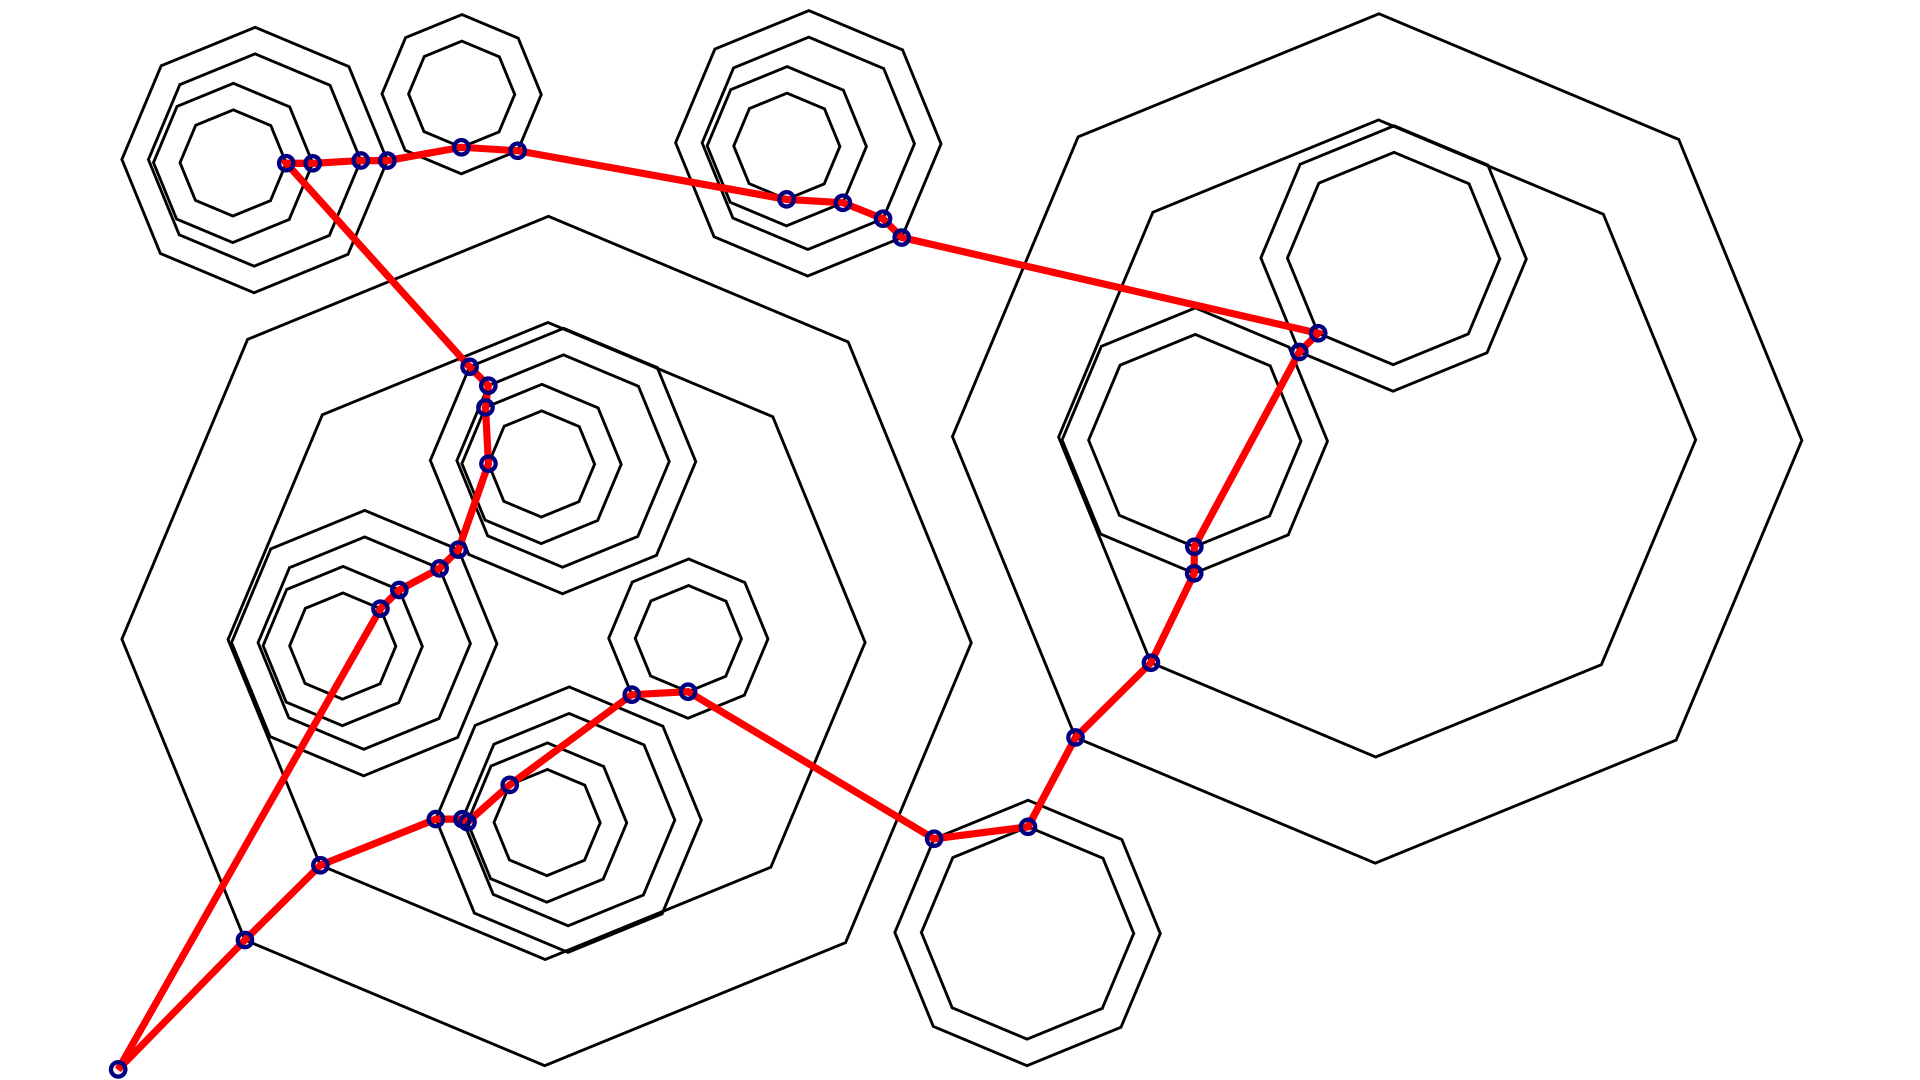
\includegraphics[width=0.95\textwidth]{34.png}
  \caption{Пример решения задачи PCGTSP, полученного эвристикой PCGLNS}
  \label{fig:pcgtsp.svg}
\end{figure}
